\documentclass{article}
\usepackage[catalan]{babel}
\usepackage[latin1]{inputenc}   % Permet usar tots els accents i car�ters llatins de forma directa.
\usepackage{enumerate}
\usepackage{amsfonts, amscd, amsmath, amssymb}
\usepackage[pdftex]{graphicx}

\setlength{\textwidth}{16cm}
\setlength{\textheight}{24.5cm}
\setlength{\oddsidemargin}{-0.3cm}
\setlength{\evensidemargin}{0.25cm} \addtolength{\headheight}{\baselineskip}
\addtolength{\topmargin}{-3cm}

\newcommand\Z{\mathbb{Z}}
\newcommand\R{\mathbb{R}}
\newcommand\N{\mathbb{N}}
\newcommand\Q{\mathbb{Q}}
\newcommand\K{\Bbbk}
\newcommand\C{\mathbb{C}}

\newcounter{exctr}
\newenvironment{exemple}
{ \stepcounter{exctr} 
\hspace{0.2cm} 
\textit{Exemple  \arabic{exctr}: }
\it
\begin{quotation}
}{\end{quotation}}


\begin{document}

\textbf{\Large Formulari PDS}

\begin{center}
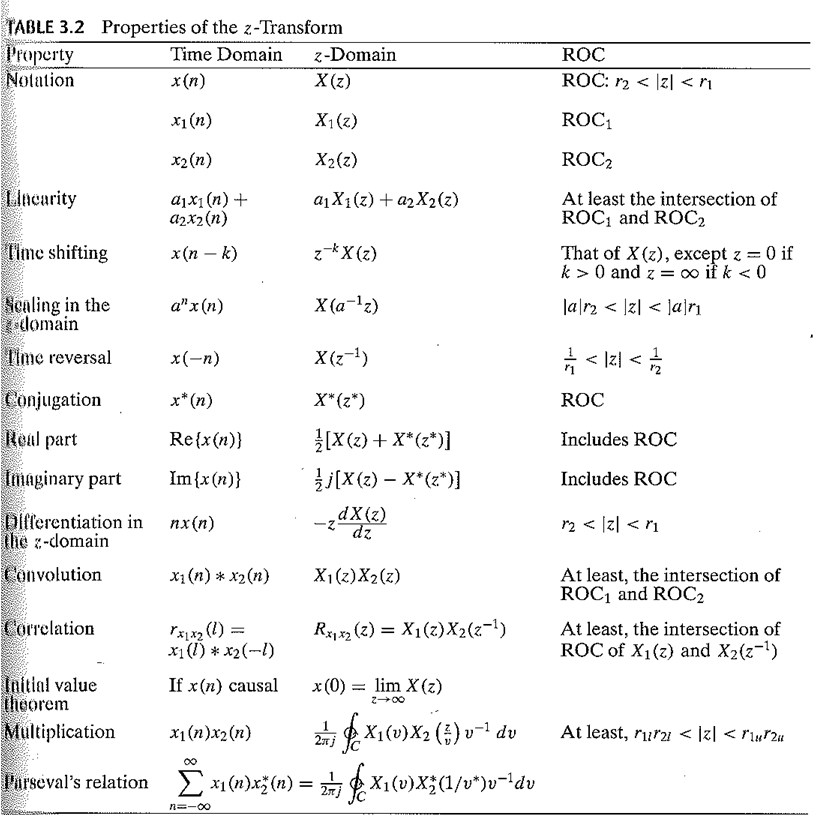
\includegraphics[width=12cm]{tabpropTZ.png}
\end{center}

\begin{center}
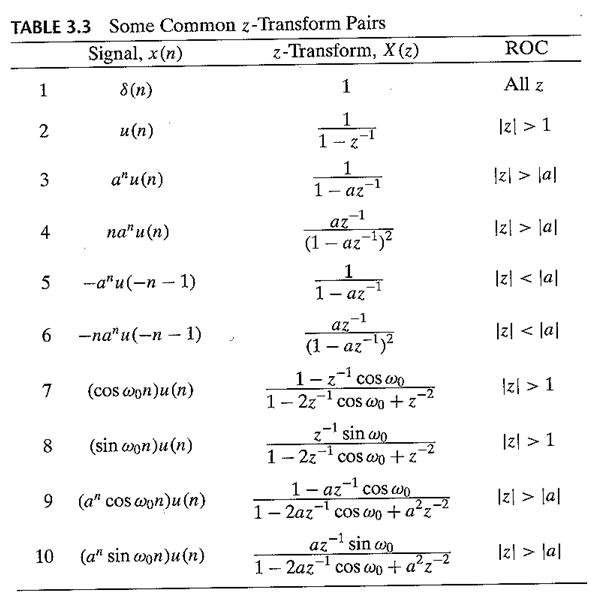
\includegraphics[width=9cm]{TZhabituals.png}
\end{center}

\begin{center}
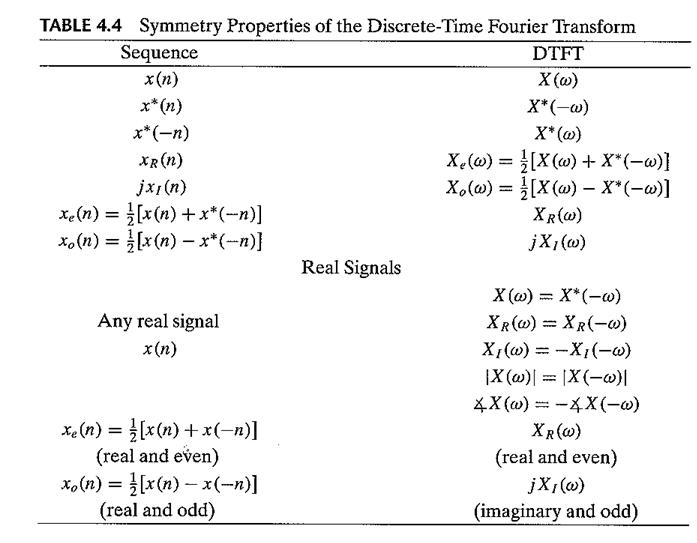
\includegraphics[width=10cm]{tabpropsimetria.png}
\end{center}

\begin{center}
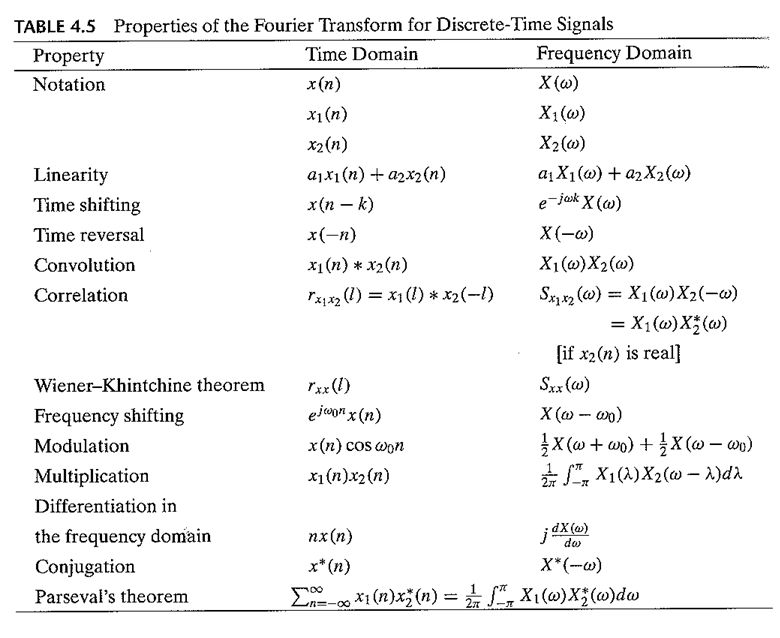
\includegraphics[width=12cm]{tabpropTF.png}
\end{center}

\begin{center}
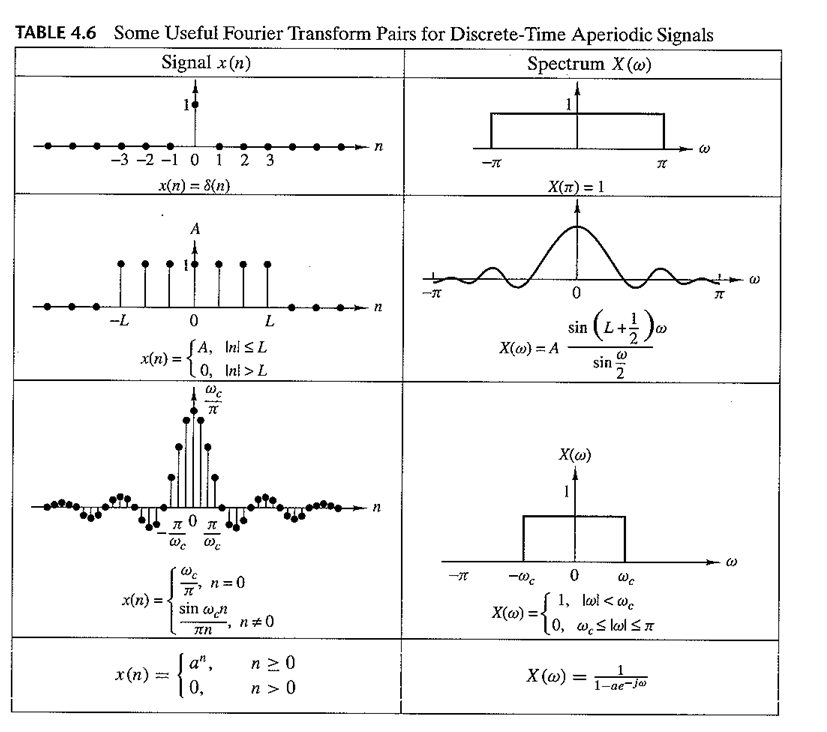
\includegraphics[width=10cm]{tabTFpairs.png}
\end{center}

\begin{center}
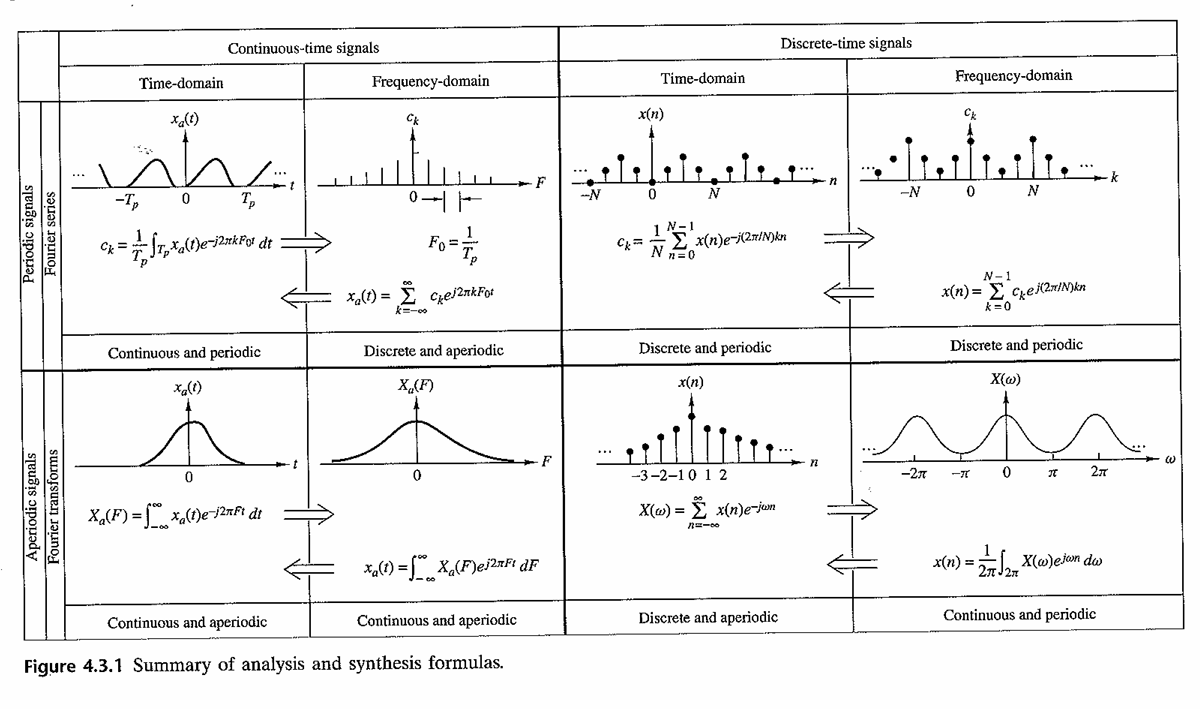
\includegraphics[width=18cm]{sumariTF2.png}
\end{center}


Font: Digital Signal Processing, J. Proakis, D. Manolakis, Pearson Prentice Hall, 2007

\end{document}